\begin{spacing}{1.5}
\section{Overview}
Results are organized around inventory coverage, fresh execution and numerical examples, followed by historical desktop and Android verification. The fresh experiments use the included sample resized to 128 by 128 pixels. They check valid outputs across the default operation path and provide selected descriptive statistics. Historical test logs remain separate evidence and are not represented as a newly repeated physical-device evaluation [8].

\section{Results}
\begin{table}[htbp]\centering\small
\caption{Verified operation inventory by registry group}
\begin{tabularx}{\textwidth}{XX}
\toprule
\textbf{Group} & \textbf{Registered operations}\\\midrule
Color \& intensity & 11\\
Geometry & 5\\
Histograms & 9\\
Filters \& restoration & 8\\
Edges \& segmentation & 11\\
Morphology & 1\\
Transforms \& comparison & 6\\
Compression & 1\\
Fundamentals & 7\\
Total & 59\\
\bottomrule\end{tabularx}\end{table}
\begin{table}[htbp]\centering\small
\caption{Course catalog chapter inventory}
\begin{tabularx}{\textwidth}{XX}
\toprule
\textbf{Chapter} & \textbf{Topic records}\\\midrule
1 Digital Image Fundamentals & 16\\
2 Image Enhancement & 15\\
3 Color Image Processing & 6\\
4 Image Transforms & 9\\
5 Image Segmentation & 16\\
6 Image Restoration & 14\\
7 Image Compression & 10\\
8 Morphological Processing & 0\\
Total & 86\\
\bottomrule\end{tabularx}\end{table}
All 59 registered operations completed the fresh default invocation with a nonempty, finite uint8 result. This checks the common execution path for the bounded sample. The output shapes vary because some operations resize images, return channel representations or compute fixed classroom matrices. The retained operation\_verification.json file records each output shape and representation. Passing this check does not prove correctness for every parameter combination or arbitrary input.

\begin{table}[htbp]\centering\small
\caption{Fresh grayscale output statistics for the 128 by 128 sample}
\begin{tabularx}{\textwidth}{XXXXX}
\toprule
\textbf{Operation} & \textbf{Mean} & \textbf{RMS contrast} & \textbf{Minimum} & \textbf{Maximum}\\\midrule
Grayscale & 147.769 & 34.875 & 68 & 200\\
Image negative & 107.231 & 34.875 & 55 & 187\\
Normalized equalization & 133.617 & 78.757 & 0 & 255\\
Adaptive equalization · CLAHE & 164.132 & 36.666 & 71 & 232\\
Median filter & 149.849 & 33.678 & 68 & 200\\
Otsu segmentation & 150.690 & 125.373 & 0 & 255\\
\bottomrule\end{tabularx}\end{table}
Table 5.3 compares output distributions under default settings. These values are descriptive: an increased standard deviation means a wider grayscale distribution, not demonstrated task improvement. Threshold output contains a binary intensity set; a negative reverses intensity ordering. Median filtering and equalization pursue different goals and should not be ranked using mean or RMS contrast alone.

\begin{table}[htbp]\centering\small
\caption{Fresh lossless coding results at the 32 pixel side setting}
\begin{tabularx}{\textwidth}{XXXXX}
\toprule
\textbf{Codec} & \textbf{Raw bytes} & \textbf{Payload bytes} & \textbf{Export bytes} & \textbf{Exact decode}\\\midrule
RLE & 1024 & 4425 & 6014 & True\\
Huffman & 1024 & 792 & 3319 & True\\
Arithmetic & 1024 & 789 & 1990 & True\\
LZW & 1024 & 1152 & 1699 & True\\
\bottomrule\end{tabularx}\end{table}
Each codec reconstructed its own grayscale analysis image exactly. Export byte counts include decoding information and JSON representation, whereas payload counts cover coded data only. Differences between the two columns show why the educational export should not be treated as a competitive general-purpose image format. LZW uses fixed 16-bit codes in this implementation [5].

\subsection{Exact Classroom Equalization}
The normalized equalization experiment contains 64 pixels and has a minimum positive cumulative count of 1. Fresh execution maps intensity 52 to 0 and intensity 55 to 12. The results agree with the specified normalized formula. The 5 by 5 histogram example separately has counts [2, 5, 3, 4, 5, 2, 4] for intensities zero through six [6].

These small examples are valuable because their expected values can be checked directly. They establish the mapping convention more clearly than judging only the appearance of a photograph. They do not substitute for checking numerical edge cases such as constant images or unsupported parameter values.

\begin{figure}[htbp]\centering
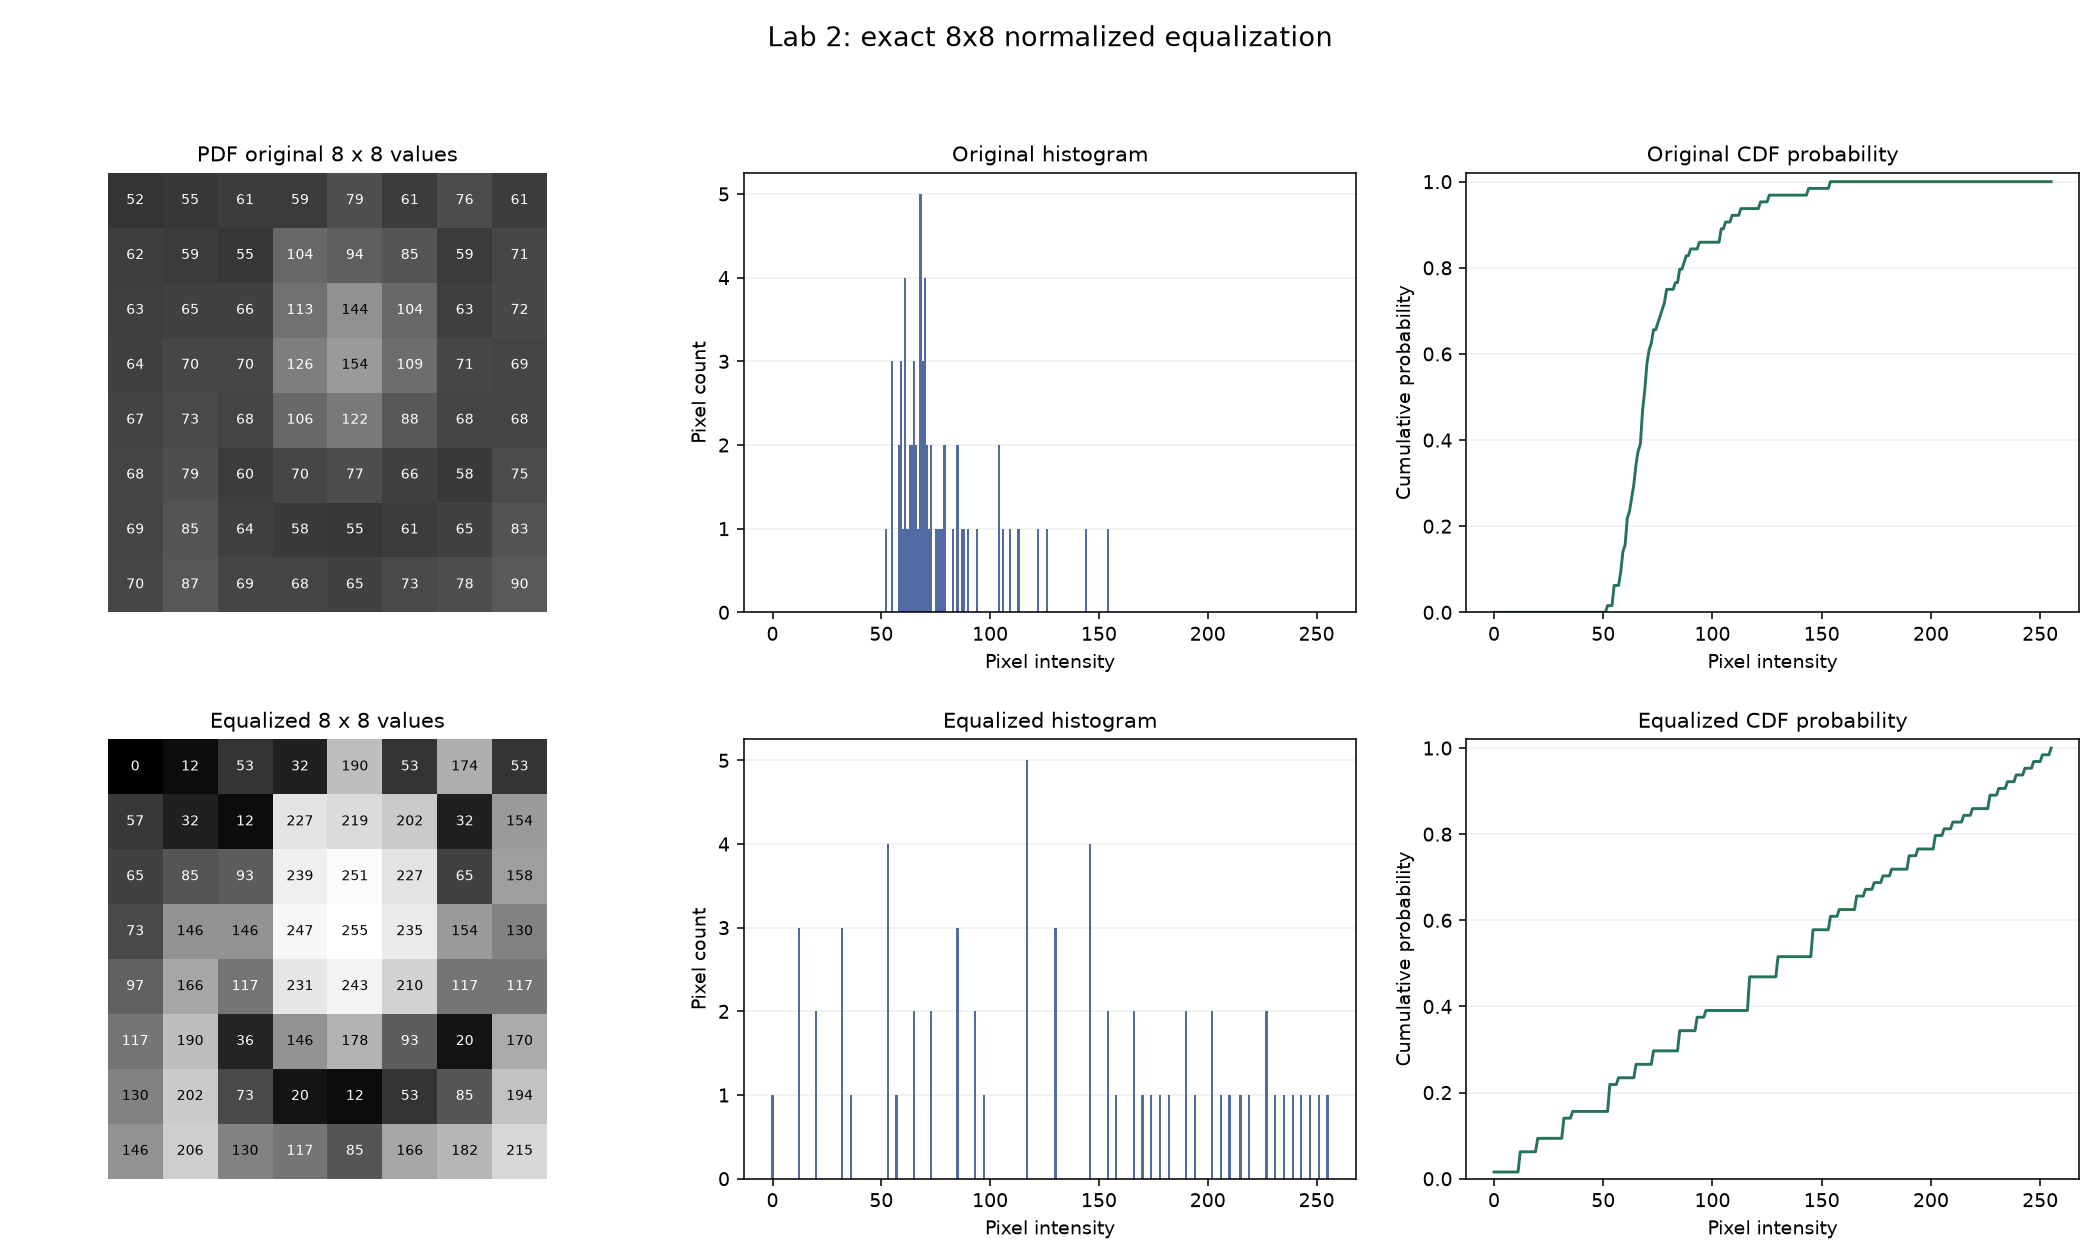
\includegraphics[width=5.6in,height=0.65\textheight,keepaspectratio]{Figures/lab_normalized_equalization_added.png}
\caption{Retained classroom normalized equalization output}
\end{figure}
\subsection{Recorded Desktop and Android Verification}
A fresh full Python suite run for this report also passed all 47 tests in 43.691 seconds. This run is separate from the bounded 59-operation execution check and from the historical Android evidence. The command was python -m unittest discover -s python\_code -p "test\_*.py".

The retained offline-host-tests.log records 47 Python tests completed successfully in 54.006 seconds. The latest retained sidebar-device-tests.log records 272 Android integration checks. Earlier logs record 193 and 266 checks for earlier verification stages; these counts are not added together because the suites overlap. Android documentation describes execution on an Android 36 x86\_64 emulator with connectivity disabled [7,8].

The Android documentation also records signature verification and visual review of the delivered APK. Source inspection independently confirms that the application manifest declares no Internet permission. A physical ARM64 phone was not available for the documented verification, even though ARM64 libraries are packaged. Test counts therefore support the specific checks and environment recorded, rather than universal device compatibility.

\begin{table}[htbp]\centering\small
\caption{Evidence mapped to project objectives}
\begin{tabularx}{\textwidth}{XX}
\toprule
\textbf{Objective} & \textbf{Evidence and interpretation}\\\midrule
Common operation interface & 59 fresh default invocations completed with valid result arrays\\
Course alignment & 86 catalog topics and original chapter and lab references\\
Explanatory output & Operation-specific plots, statistics, tables and examples in source and retained views\\
Offline Android execution & Embedded Python bridge, bundled libraries and recorded emulator checks\\
Numerical verification & Exact equalization values, codec round trips and retained automated suites\\
\bottomrule\end{tabularx}\end{table}
\section{Detailed Analysis}
The implementation meets the main integration objectives: one operation inventory supports a consistent experiment workflow, while the course catalog supplies navigation and references. Grouped operations reduce interface repetition but require precise reporting of coverage. For example, one lossless operation exposes four codecs, and one noise operation exposes several distributions. Reporting 59 operations as 59 independent algorithms would understate some families and misdescribe the structure.

The educational matrices and uploaded-image workflows serve different purposes. Exact matrices support step-by-step numerical reasoning. Uploaded images reveal sensitivity to texture, illumination, color and scale. The system retains both without treating the classroom examples as a representative dataset. Similarly, a display-normalized spectrum demonstrates frequency content but does not preserve all information required for inverse transformation.

The mobile implementation removes the running-server requirement from the installed application. Its feasibility is supported by direct embedding and recorded emulator checks. However, scientific libraries increase package size and resource demands. A 12-million-pixel input limit restricts one dimension of memory exposure, but operations may allocate multiple arrays. Input limits alone are not evidence of low memory consumption on every supported device.

Learning outcomes and comparative usability require separate studies using explicit tasks and representative devices.

\end{spacing}